\documentclass{standalone}

\usepackage[euler-digits]{eulervm}

\usepackage{tikz}
\tikzset{every node/.style={circle,align=center,draw,shade,minimum size=6mm,inner sep=0pt}}
\tikzset{every path/.style={->,>=latex}}
\tikzset{t/.style={rectangle}}
\tikzset{r/.style={top color=red}}
\tikzset{g/.style={top color=green}}
\tikzset{b/.style={top color=blue}}

\usetikzlibrary{shapes}

\begin{document}
    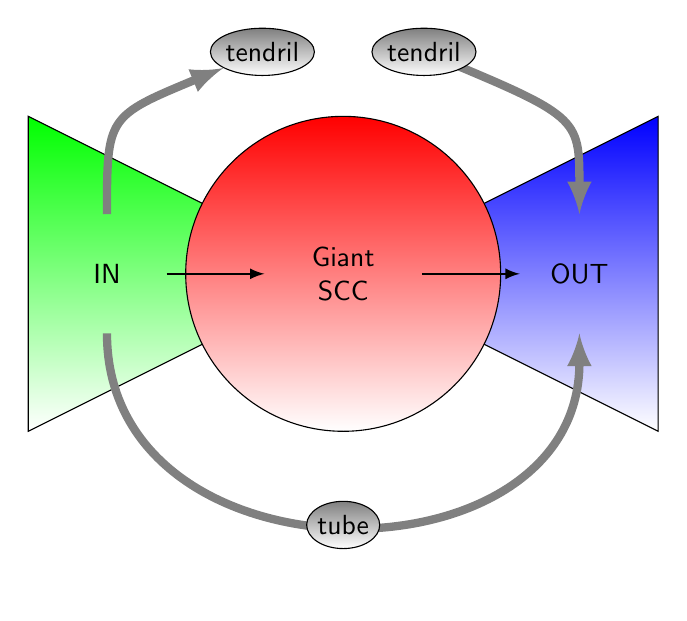
\begin{tikzpicture}[font=\sffamily]
\fill[draw,shade,top color=blue] (0,0)--(4,2)--(4,-2) -- cycle;
\fill[draw,shade,top color=green] (0,0)--(-4,2)--(-4,-2) -- cycle;
\node[r,minimum size=4cm](SCC) at (0,0) {Giant\\SCC};
\node[draw=none,shade=none,minimum size=1.5cm] (I) at (-3,0) {IN};
\node[draw=none,shade=none,minimum size=1.5cm] (O) at (3,0) {OUT};
\node[thin,ellipse,black] (tendril) at (110:3) {tendril};
\draw[thick] (I) -- (-1,0);
\draw[thick] (1,0) -- (O);
\draw[line width=3pt,black!50] (I) .. controls (-3,-4) and (3,-4) .. node[thin,ellipse,black] {tube} (O);
\draw[line width=3pt,black!50] (I) .. controls (-3,2) ..  (tendril);
\draw[line width=3pt,black!50] (70:3) node[thin,ellipse,black] {tendril} .. controls (3,2) .. (O) ;
    \end{tikzpicture}
\end{document}
